\documentclass[11pt,a4paper]{article}
\usepackage[margin=2.5cm]{geometry}
\usepackage{booktabs,graphicx,amsmath,hyperref,float,caption,setspace}
\hypersetup{colorlinks=true,linkcolor=black,citecolor=black,urlcolor=blue}
\setstretch{1.12}
\graphicspath{{figures/}{./}}
\title{Two-Stage Machine-Learning Screening of Earth-Abundant Semiconductor Absorbers from Composition: Accuracy, Limits Across Anion Families, and Window Probabilities}
\author{%
Priom Dey$^{*}$, Avro Talukder, Yuvraj Roy\\[4pt]
\small Department of Chemistry, Shahjalal University of Science and Technology, Sylhet, Bangladesh\\[4pt]
\small $^{*}$Corresponding author: \texttt{2023131044@student.sust.edu}\\[2pt]
\small P.~Dey: ORCID \href{https://orcid.org/0009-0007-5722-8240}{0009-0007-5722-8240}\\
\small A.~Talukder: \texttt{2023131055@student.sust.edu}, ORCID \href{https://orcid.org/0009-0007-6996-7673}{0009-0007-6996-7673}\\
\small Y.~Roy: \texttt{2023131056@student.sust.edu}}
\date{}
\begin{document}\sloppy\maketitle

\begin{abstract}
Low-cost electronics and photovoltaics need semiconductors made of abundant elements, but experimental screening is slow.
We trained random-forest models on 4604 experimental band gaps (Matbench \texttt{expt\_gap}) and compared a single-stage regressor with a two-stage model that first classifies a compound as metal or non-metal and then predicts the gap of non-metals. Under cross-validation that withholds whole chemical systems, the two-stage model lowered the mean absolute error (MAE) over all compounds from 0.474 to 0.384~eV (paired difference 0.090~eV, 95\% CI 0.073 to 0.108). The gain came from the metal/non-metal decision (accuracy 90.7\%); for true non-metals the two models were not clearly different (0.599 vs.\ 0.584~eV).
Accuracy depended strongly on anion family: regressor MAE was 0.335~eV for chalcogenides, 0.444~eV for pnictides, 0.694~eV for oxides and 0.877~eV for halides. When an entire anion family was withheld, the regressor MAE on non-metals was 0.604~eV for pnictides and 0.631~eV for chalcogenides but 1.470~eV for oxides and 1.739~eV for halides, and the two-stage rule was worse than the single-stage model for non-metals (1.487 vs.\ 1.058~eV).
Out-of-fold residuals were converted into the probability that a predicted gap lies in the 1.0--1.8~eV single-junction window. On held-out chalcogenides and pnictides this probability was reasonably calibrated (Brier skill score 0.23), and the top 5\% by probability had a precision of 73.2\% against a base rate of 23.2\% (enrichment 3.16). Applied to 8,326 Materials Project compounds made only of abundant elements outside our toxicity and cost exclusion lists, it gave 98 candidates with a probability of at least 0.30 (maximum 0.59), several of them already studied photovoltaic absorbers.
For 12 chalcogenides and pnictides with measured literature gaps the MAE was 0.34~eV; all 8 compounds with a probability of at least 0.30 lie in the window, but two in-window zirconium sulfide perovskites were missed.
The results support composition-only screening as a coarse filter for chalcogenides and pnictides, but not for oxides or for unseen anion families, and they do not show that any candidate will work in a device.
\end{abstract}
\noindent\textbf{Keywords:} band gap; machine learning; earth-abundant semiconductors; photovoltaics; materials screening; model validation

\section{Introduction}
The band gap largely determines whether a material is useful as a light absorber, a transparent conductor or an insulator.
Cheap solar cells and low-cost electronics therefore motivate a search for semiconductors that avoid scarce, costly or toxic elements. First-principles calculations
with standard density functionals systematically underestimate gaps and are expensive, which has led to machine-learning models trained directly on experimental
gaps using composition alone \cite{Zhuo2018,Ward2016}. Standard benchmarks such as Matbench allow such models to be compared on common data \cite{Dunn2020}.

Three practical issues are less often quantified. First, experimental data sets contain many metals with a recorded gap of zero, and a single regressor must blend them with semiconductors.
Second, random cross-validation can overstate performance when related compounds appear on both sides of a split, and performance on new chemistries may be lower \cite{Meredig2018}.
Third, a screening user needs to know how likely a predicted gap is to fall in a useful window, not only a point estimate.

This study addresses these issues on a public data set with free software. We (i) compare single-stage and two-stage models under chemical-system cross-validation with intervals that resample whole chemical systems;
(ii) report accuracy per anion family and under a stress test that withholds an entire family; (iii) convert out-of-fold errors into a probability of lying in the 1.0--1.8~eV window, test its calibration and its enrichment of in-window compounds on held-out data, and apply it to real,
low-cost candidate compounds; and (iv) check predictions against measured gaps of 12 compounds compiled from the literature. We do not claim to have discovered a new solar absorber; a suitable gap is necessary but far from sufficient for a working device.

\section{Data and Methods}
\subsection{Experimental band-gap data}
We used the \texttt{matbench\_expt\_gap} data set distributed with \texttt{matminer} \cite{Ward2018matminer,Dunn2020}, derived from the compilation of Zhuo et al.\ \cite{Zhuo2018}:
4604 inorganic compositions with experimental gaps in eV, of which 46.8\% are non-metals (gap~$>0$) and the rest have a recorded gap of exactly zero. No rows were removed or altered.
The compounds fall into 3705 distinct chemical systems (a chemical system is the set of elements in a compound), so most systems contain a single compound. Composition cannot encode polymorph, defects,
temperature, or whether a value is optical or fundamental; this label noise is irreducible here. Compounds were assigned to an anion family by priority: oxide (contains O), chalcogenide (S, Se or Te), halide, pnictide (N, P, As or Sb), otherwise ``other'' (mainly metals and intermetallics).

\subsection{Features and models}
Compositions were converted to the Magpie elemental-property descriptors (132 features) with \texttt{pymatgen} and \texttt{matminer} \cite{Ong2013,Ward2018matminer,Ward2016}.
All models were random forests \cite{Breiman2001} from \texttt{scikit-learn} \cite{Pedregosa2011} with fixed settings (200 trees in cross-validation, 300 in final models; no tuning).
The \emph{single-stage} model regresses the gap on all compounds. The \emph{two-stage} model uses a random-forest classifier for metal vs.\ non-metal and a random-forest regressor trained on non-metals only;
a compound is predicted to have gap zero if the classifier's non-metal probability is 0.5 or lower, otherwise the regressor's value.

\subsection{Evaluation}
Main results use five-fold cross-validation in which every chemical system lies wholly in one fold (assignment by a seeded, size-balanced procedure; disjointness was asserted in code).
For comparison we also report ordinary shuffled five-fold cross-validation with a fixed seed, and a stress test in which one anion family at a time (chalcogenide, halide, oxide, pnictide) is withheld entirely, with the ``other'' family always kept in training.
We report MAE and, for metal/non-metal classification, accuracy and the area under the ROC curve. Because compounds within a system are correlated, 95\% intervals come from a bootstrap that resamples whole chemical systems (2000 resamples).
The paired difference between models uses the same resampled systems.

\subsection{Low-cost candidate set}
Candidates were restricted to the 26 common elements listed in Table~\ref{tab:abund} (rounded crustal abundances following \cite{CRC}), all of which have an abundance of at least 2~ppm. None is on our toxicity exclusion list (Pb, Cd, As, Se, Hg, Tl, Be) or our scarce-or-costly list (Te, In, Ga, Ge, Sb, Bi, Ag, Co). Other elements with abundance above 2~ppm (for example B, Y, Nb, Rb and the lanthanides) were not considered. Cr, Ni, V and Ba were not excluded although some of their compounds are hazardous; both lists are judgements (see Limitations).
Candidate compounds were taken from the Materials Project \cite{Jain2013} (via the \texttt{matbench\_mp\_e\_form} data set): reduced formulas with negative formation energy (the lowest value across polymorphs),
made only of allowed elements, containing at least one of O, S, N or P, no halogen, at most four elements, and not present in the experimental training set by composition.
Negative formation energy is only a rough stability screen; it does not guarantee stability against decomposition. The allowed elements were therefore Al, Ba, Br, Ca, Cl, Cr, Cu, F, Fe, K, Li, Mg, Mn, N, Na, Ni, O, P, S, Si, Sn, Sr, Ti, V, Zn, Zr (Br, Cl and F are in the list but, by the rule above, no halogen-containing compound was kept).

\subsection{Probability of lying in the target window}
Single-junction photovoltaic absorbers are most efficient for gaps of roughly 1.0--1.8~eV, centred near 1.3--1.4~eV \cite{SQ1961}; we used 1.0--1.8~eV as the target window.
For a candidate with predicted non-metal probability $p$ and regressor prediction $g$, the probability of lying in the window was estimated as
$p \times \frac{1}{n}\sum_i \mathbf{1}[1.0 \le g + r_i \le 1.8]$, where $r_i$ are the out-of-fold residuals of the regressor on true non-metals under the chemical-system protocol.
This assumes that a candidate's error resembles the out-of-fold errors, which is least likely to hold for chemistries unlike the training data.
The 90th percentile of absolute out-of-fold error was 1.03~eV.

\subsection{Calibration, enrichment, stability and baselines}
To test whether the window probability is useful, each outer training set was split by chemical system into a proper-training set (80\%) and a calibration set (20\%); models were fitted on the proper-training set, calibration residuals defined the probabilities, and only the held-out fold was scored.
A compound is \emph{truly in the window} if its measured gap lies in 1.0--1.8~eV (metals, with gap zero, are not). We report the Brier score against a constant base-rate forecast (Brier skill score), the ROC AUC, a reliability table, and the \emph{enrichment}: the precision among the top 2\%, 5\% and 10\% of compounds ranked by window probability divided by the base rate.
Two naive rankings serve as comparison: closeness of the single-stage (or two-stage) predicted gap to 1.4~eV. The whole procedure was repeated for 3 different assignments of systems to folds (seeds 42--44). We compared random forest with histogram gradient boosting (300 iterations, learning rate 0.05) for the non-metal gap regressor.

\section{Results}
\subsection{Single-stage versus two-stage under chemical-system folds}\label{sec:single}
Table~\ref{tab:main} gives the main results and Fig.~\ref{fig:parity} shows predictions. The two-stage model lowered the MAE over all compounds from 0.474 to 0.384~eV
(difference 0.090~eV, 95\% CI 0.073 to 0.108). Metal/non-metal accuracy was 90.7\% (ROC AUC 0.967). For compounds that are truly non-metals, however, the two-stage MAE (0.584~eV) and the single-stage MAE (0.599~eV) had overlapping 95\% intervals, so we find no clear gain in gap accuracy for non-metals; the improvement comes from avoiding the blending of metals and semiconductors.
Fig.~\ref{fig:parity} also shows the cost of the hard rule: non-metals misclassified as metals appear as predictions of exactly zero.
Ordinary shuffled folds gave a single-stage MAE of 0.463~eV against 0.474~eV for system folds, a negligible difference, because 3705 systems share 4604 compounds and system grouping removes little related information;
chemical-system folds are therefore not a strict test of transfer to new chemistry (Table~\ref{tab:prot}).

\begin{table}[H]\centering\small\caption{Chemical-system cross-validation (eV; 95\% intervals resample whole chemical systems).}\label{tab:main}
\begin{tabular}{lc}\toprule Quantity & Value [95\% CI]\\\midrule
MAE, all compounds, single-stage & 0.474 [0.452, 0.496] \\
MAE, all compounds, two-stage & 0.384 [0.359, 0.410] \\
Difference (single $-$ two-stage) & 0.090 [0.073, 0.108] \\
MAE, true non-metals, single-stage & 0.599 [0.561, 0.637] \\
MAE, true non-metals, two-stage & 0.584 [0.544, 0.628] \\
MAE, true non-metals, regressor given non-metal & 0.458 [0.434, 0.483] \\
Metal/non-metal accuracy & 0.907 [0.898, 0.915] \\
\bottomrule\end{tabular}\end{table}

\begin{figure}[H]\centering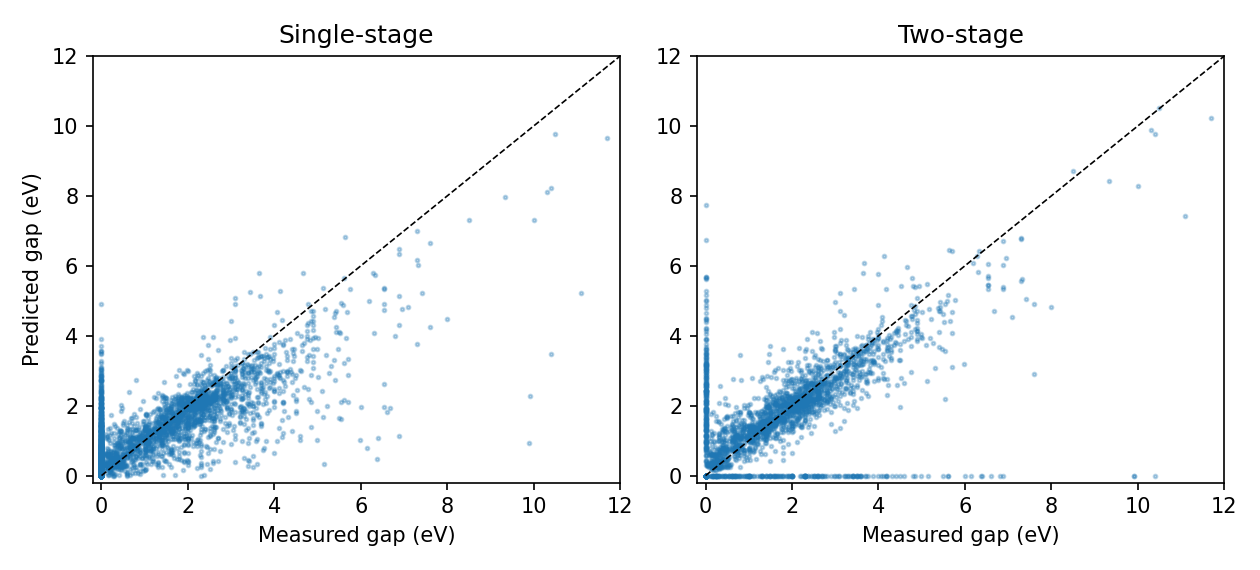
\includegraphics[width=.9\linewidth]{fig1_single_vs_two_stage.png}\caption{Out-of-fold predictions under chemical-system folds for the single-stage and two-stage models.}\label{fig:parity}\end{figure}

\subsection{Dependence on anion family}
Table~\ref{tab:fam} reports performance by family under chemical-system folds. The regressor error on non-metals was lowest for chalcogenides (0.335~eV) and pnictides (0.444~eV) and higher for oxides (0.694~eV) and halides (0.877~eV).
For oxides only 84.2\% of compounds were correctly classified as metal or non-metal, and the two-stage MAE on oxide non-metals was 1.049~eV, much larger than the regressor error given the correct class.

\begin{table}[H]\centering\small\caption{Per-family results under chemical-system folds. MAE (eV) of the regressor on true non-metals with 95\% CI; last column is the two-stage MAE on true non-metals.}\label{tab:fam}
\begin{tabular}{lccccc}\toprule Family & $n$ & Non-metal share & Class.\ accuracy & Regressor MAE [95\% CI] & Two-stage MAE\\\midrule
chalcogenide & 1485 & 0.87 & 0.923 & 0.335 [0.314, 0.358] & 0.347 \\
pnictide & 425 & 0.47 & 0.854 & 0.444 [0.370, 0.528] & 0.539 \\
oxide & 1090 & 0.45 & 0.842 & 0.694 [0.634, 0.758] & 1.049 \\
halide & 177 & 0.44 & 0.825 & 0.877 [0.656, 1.138] & 1.513 \\
other & 1427 & 0.07 & 0.966 & 0.595 [0.490, 0.760] & 0.736 \\
\bottomrule\end{tabular}\end{table}

\subsection{Protocol comparison and withholding an entire anion family}
Table~\ref{tab:prot} compares three protocols. Withholding a whole anion family is much harder: classification accuracy fell to 0.687 (AUC 0.810), and the two-stage MAE on non-metals (1.487~eV) was larger than the single-stage MAE (1.058~eV).
Table~\ref{tab:fh} gives the family-by-family result: when chalcogenides or pnictides were withheld the regressor MAE on non-metals was 0.631 and 0.604~eV, but 1.470~eV for oxides and 1.739~eV for halides.
Predictions should therefore not be trusted for anion families absent from the training data.

\begin{table}[H]\centering\footnotesize\setlength{\tabcolsep}{3.5pt}\caption{Evaluation protocols (eV). ``Family'' withholds one anion family at a time; ``other'' is always kept in training and not scored. NM = true non-metals; Reg.\ = regressor given a non-metal.}\label{tab:prot}
\begin{tabular}{lcccccccc}\toprule Protocol & $n$ tested & MAE single & MAE two-stage & NM single & NM two-stage & NM Reg. & Accuracy & AUC\\\midrule
random & 4604 & 0.463 & 0.371 & 0.572 & 0.554 & 0.436 & 0.911 & 0.969 \\
system & 4604 & 0.474 & 0.384 & 0.599 & 0.584 & 0.458 & 0.907 & 0.967 \\
family & 3177 & 1.066 & 1.036 & 1.058 & 1.487 & 0.870 & 0.687 & 0.810 \\
\bottomrule\end{tabular}\end{table}

\begin{table}[H]\centering\small\caption{Withholding one anion family at a time.}\label{tab:fh}
\begin{tabular}{lcccc}\toprule Held-out family & $n$ & Non-metals & Regressor MAE (eV) & Class.\ accuracy\\\midrule
chalcogenide & 1485 & 1291 & 0.631 & 0.712 \\
pnictide & 425 & 199 & 0.604 & 0.772 \\
oxide & 1090 & 491 & 1.470 & 0.613 \\
halide & 177 & 77 & 1.739 & 0.740 \\
\bottomrule\end{tabular}\end{table}

\subsection{Calibration and enrichment of the window probability}\label{sec:cal}
Averaged over 3 cross-validation seeds, the Brier skill score of the window probability relative to a constant base-rate forecast was 0.234 $\pm$ 0.004 for chalcogenides and pnictides and 0.300 $\pm$ 0.004 for all compounds, and the ROC AUC for identifying in-window compounds was 0.818 $\pm$ 0.002 and 0.898 $\pm$ 0.002, respectively (Table~\ref{tab:cal}). In the reliability table for chalcogenides and pnictides (Table~\ref{tab:rel}, Fig.~\ref{fig:rel}), predicted and observed frequencies differed by at most 0.13 in any bin; the highest-probability bin had a mean predicted probability of 0.54 against an observed frequency of 0.67, so the probabilities were reasonably calibrated but not exact.

\begin{table}[H]\centering\small\caption{Skill of the window probability on held-out compounds (mean $\pm$ s.d.\ over 3 seeds). Brier scores: lower is better; AUC for identifying in-window compounds.}\label{tab:cal}
\begin{tabular}{lccccc}\toprule Subset & Base rate & Brier & Brier (constant) & Brier skill score & AUC\\\midrule
all compounds & 11.0\% & 0.069 $\pm$ 0.000 & 0.098 $\pm$ 0.000 & 0.300 $\pm$ 0.004 & 0.898 $\pm$ 0.002 \\
chalcogenides and pnictides & 23.2\% & 0.136 $\pm$ 0.001 & 0.178 $\pm$ 0.000 & 0.234 $\pm$ 0.004 & 0.818 $\pm$ 0.002 \\
\bottomrule\end{tabular}\end{table}

\begin{table}[H]\centering\small\caption{Reliability table for chalcogenides and pnictides (seed 42): compounds sorted by predicted window probability into equal-count bins.}\label{tab:rel}
\begin{tabular}{cccc}\toprule Bin & $n$ & Mean predicted & Observed fraction\\\midrule
1 & 239 & 0.023 & 0.029 \\
2 & 239 & 0.066 & 0.033 \\
3 & 238 & 0.110 & 0.092 \\
4 & 239 & 0.163 & 0.151 \\
5 & 239 & 0.231 & 0.155 \\
6 & 238 & 0.327 & 0.294 \\
7 & 239 & 0.438 & 0.431 \\
8 & 239 & 0.541 & 0.669 \\
\bottomrule\end{tabular}\end{table}

\begin{figure}[H]\centering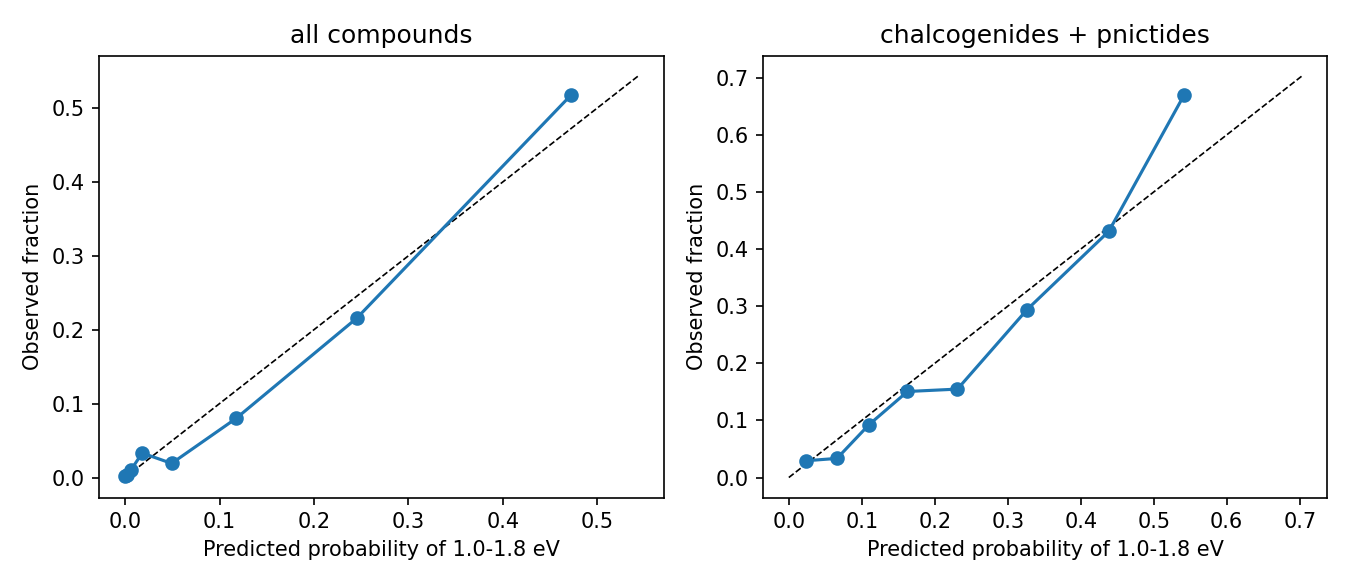
\includegraphics[width=.95\linewidth]{fig_reliability.png}\caption{Reliability of the window probability (seed 42). Dashed line: perfect calibration.}\label{fig:rel}\end{figure}

Among chalcogenides and pnictides, 23.2\% of compounds have a measured gap in the window. Selecting the 5\% of compounds with the highest window probability gave a precision of 0.73, an enrichment of 3.16 over random selection (seed-42 bootstrap 95\% CI 2.81 to 3.75). The naive ranking by closeness of the single-stage prediction to 1.4~eV gave 2.59 and the same ranking with the two-stage model gave 2.69. The window-probability ranking had the higher enrichment in 3 of 3 seeds against the first naive ranking and in 2 of 3 against the second, so its advantage over the single-stage ranking is clearer than over the two-stage ranking. For all compounds the enrichment is higher (5.92) mainly because only 11.0\% of compounds lie in the window, most of the rest being metals that the first stage removes; the value for chalcogenides and pnictides is the relevant one for screening.

\begin{table}[H]\centering\footnotesize\caption{Precision and enrichment of the top 5\% of compounds by each ranking (naive rankings sort by closeness of the predicted gap to 1.4~eV) (mean $\pm$ s.d.\ over 3 seeds).}\label{tab:enr}
\begin{tabular}{llcc}\toprule Subset & Ranking & Precision & Enrichment\\\midrule
all compounds & Window probability & 0.652 $\pm$ 0.020 & 5.92 $\pm$ 0.18 \\
all compounds & Naive 1.4~eV, single-stage & 0.437 $\pm$ 0.028 & 3.97 $\pm$ 0.26 \\
all compounds & Naive 1.4~eV, two-stage & 0.610 $\pm$ 0.034 & 5.54 $\pm$ 0.31 \\
chalcogenides and pnictides & Window probability & 0.732 $\pm$ 0.026 & 3.16 $\pm$ 0.12 \\
chalcogenides and pnictides & Naive 1.4~eV, single-stage & 0.601 $\pm$ 0.034 & 2.59 $\pm$ 0.14 \\
chalcogenides and pnictides & Naive 1.4~eV, two-stage & 0.625 $\pm$ 0.095 & 2.69 $\pm$ 0.41 \\
\bottomrule\end{tabular}\end{table}

\begin{figure}[H]\centering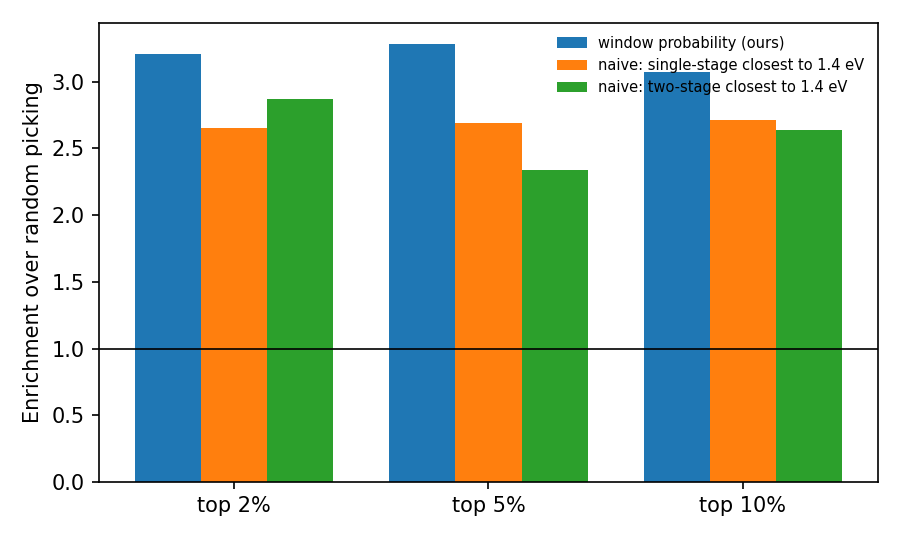
\includegraphics[width=.65\linewidth]{fig_enrichment.png}\caption{Enrichment over random selection for chalcogenides and pnictides (seed 42).}\label{fig:enr}\end{figure}

\subsection{Stability across splits and baseline regressors}
Across 3 different assignments of chemical systems to folds the MAE over all compounds was 0.476 $\pm$ 0.005~eV (single-stage) and 0.384 $\pm$ 0.007~eV (two-stage), and for true non-metals 0.598 $\pm$ 0.003 and 0.586 $\pm$ 0.013~eV; metal/non-metal accuracy was 0.908 $\pm$ 0.003. The conclusions of Section~\ref{sec:single} were therefore not sensitive to the fold assignment. For the gap regressor on non-metals, gradient boosting (MAE 0.441~eV) and random forest (0.458~eV) had overlapping 95\% intervals (Table~\ref{tab:base}). A ridge-regression baseline was numerically unstable on compositions unlike the training fold and is omitted.

\begin{table}[H]\centering\small\caption{Non-metal gap regressors under chemical-system folds (seed 42): MAE on true non-metals (eV) with 95\% CI.}\label{tab:base}
\begin{tabular}{lc}\toprule Regressor & MAE [95\% CI]\\\midrule
Random forest (used) & 0.458 [0.434, 0.483] \\
Gradient boosting & 0.441 [0.418, 0.466] \\
\bottomrule\end{tabular}\end{table}

\subsection{Low-cost candidates}
The candidate set contained 8,326 compounds. Table~\ref{tab:cf} gives counts by family and Table~\ref{tab:top} lists the twelve chalcogenide and pnictide candidates with the highest estimated probability of lying in the 1.0--1.8~eV window.
The highest probability was 0.59, and 98 candidates exceeded 0.30 (Fig.~\ref{fig:hist}). Even the best candidates carry a large chance of lying outside the window. Several top-ranked candidates (SnS, Cu$_2$SnS$_3$, Cu$_2$FeSnS$_4$, ZnSnP$_2$) are already studied photovoltaic absorbers \cite{Reddy2006,Marquez2016,Hou2017,StJean2010}. This is a useful sanity check on the ranking, but it means the list should not be read as a set of discoveries; the less studied entries are hypotheses only. Candidates that are oxides are not tabulated:
the per-family results above show that oxide predictions are unreliable, and the eight highest-ranked oxides (all chromium or manganese oxides) had non-metal probabilities of only 0.49--0.73.

\begin{table}[H]\centering\small\caption{Candidate counts by family.}\label{tab:cf}
\begin{tabular}{lccc}\toprule Family & Candidates & $P\ge 0.30$ & Maximum $P$\\\midrule
chalcogenide & 685 & 60 & 0.59 \\
oxide & 6945 & 5 & 0.43 \\
pnictide & 696 & 33 & 0.54 \\
\bottomrule\end{tabular}\end{table}

\begin{table}[H]\centering\small\caption{Highest-ranked chalcogenide and pnictide candidates: predicted gap (eV), non-metal probability, probability of lying in 1.0--1.8~eV, and formation energy (eV/atom). $^\dagger$ Also in Table~\ref{tab:lit}.}\label{tab:top}
\begin{tabular}{lccccc}\toprule Formula & Family & Pred.\ gap & $P$(non-metal) & $P$(window) & $E_\mathrm{form}$\\\midrule
SnS$^\dagger$ & chalcogenide & 1.40 & 0.99 & 0.59 & -0.78 \\
Cu4Sn15S32 & chalcogenide & 1.57 & 1.00 & 0.58 & -0.72 \\
Cu(SnS2)4 & chalcogenide & 1.34 & 0.98 & 0.58 & -0.76 \\
ZnSnP2 & pnictide & 1.61 & 0.97 & 0.54 & -0.19 \\
Cu2SnS3$^\dagger$ & chalcogenide & 1.34 & 0.91 & 0.54 & -0.66 \\
Cu2P7 & pnictide & 1.37 & 0.89 & 0.53 & -0.10 \\
CuP10 & pnictide & 1.54 & 0.87 & 0.51 & -0.04 \\
SnP & pnictide & 1.21 & 0.94 & 0.51 & -0.00 \\
MnCu2Sn3S8 & chalcogenide & 1.54 & 0.84 & 0.50 & -0.78 \\
VCuSnS4 & chalcogenide & 1.50 & 0.82 & 0.49 & -0.94 \\
CrCuSnS4 & chalcogenide & 1.57 & 0.84 & 0.49 & -0.89 \\
KZn4P3 & pnictide & 1.53 & 0.81 & 0.48 & -0.30 \\
\bottomrule\end{tabular}\end{table}

\begin{figure}[H]\centering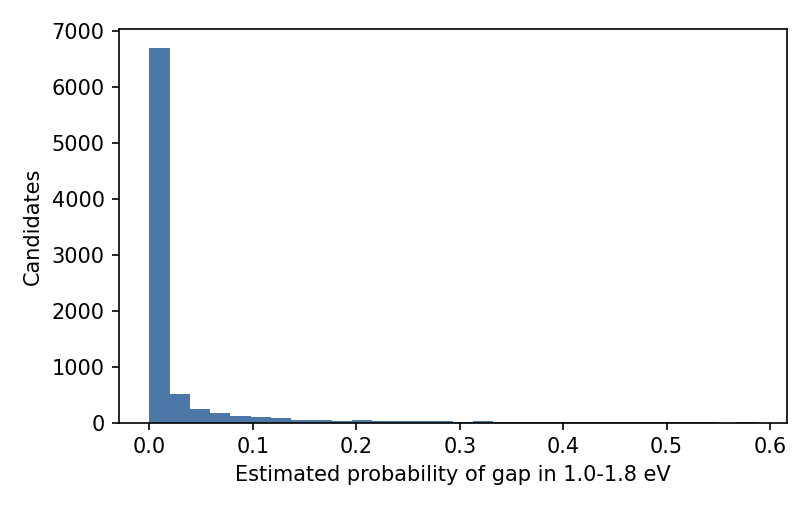
\includegraphics[width=.6\linewidth]{fig2_probability_hist.png}\caption{Distribution of the estimated probability that a candidate's gap lies in 1.0--1.8~eV.}\label{fig:hist}\end{figure}

\subsection{Comparison with measured literature gaps}
We compiled measured gaps for compounds that are absent from the training set by composition and that appear among the 8,326 candidates; twelve compounds had a usable value (Table~\ref{tab:lit}, Fig.~\ref{fig:lit}). The first four (SnS, Cu$_2$SnS$_3$, Cu$_2$FeSnS$_4$, FePS$_3$) were checked first and were chosen from the top 30 of the ranking; the other eight were added from the same compilation whatever their rank (4 to 433). Where a source reports several values their mean is shown. The Cu$_2$SnS$_3$ value is an estimate from quantum-efficiency measurements on a solar cell rather than an absorption gap \cite{Marquez2016}, and other reports for this compound range from about 0.9 to 1.65~eV. The compilation targeted photovoltaic-relevant materials, so 10 of 12 lie inside the 1.0--1.8~eV window and this fraction is not comparable with the base rates in Section~\ref{sec:cal}.

The MAE was 0.34~eV (bootstrap 95\% interval 0.19 to 0.51~eV) and 10 of 12 predictions were within 0.5~eV, comparable with the cross-validated regressor error for chalcogenides and pnictides. The first four are the most favourable (MAE 0.10~eV); the other eight have an MAE of 0.46~eV, so the first four overstate typical accuracy. Errors were largest for the zirconium chalcogenide perovskites (BaZrS$_3$, SrZrS$_3$, CaZrS$_3$), whose gaps were overestimated by 0.3 to 0.75~eV, and for MnPS$_3$, which was underestimated by 1.0~eV although the literature values for it disagree (1.7--2.8~eV). All 8 compounds with a window probability of at least 0.30 lie in the window, but BaZrS$_3$ and SrZrS$_3$, which also lie in the window, received only 0.13 and ranked about 430th. The screen can therefore miss true positives, in line with the finding that it is a coarse filter. Only 3 of the 12 compounds have a chemical system that also occurs in the training data, so most of the comparison involves unseen chemical systems, although all are chalcogenides or pnictides, i.e.\ families that are represented in the training set. With $n=12$ and a selected compilation the comparison is indicative only.

\begin{table}[H]\centering\small\caption{Predictions against measured literature gaps (eV) for compounds absent from the training set by composition, ordered by rank among the 8,326 candidates (by window probability).}\label{tab:lit}
\begin{tabular}{lcccccc}\toprule Formula & Measured & Predicted & $P$(window) & $|$Error$|$ & Rank & Source\\\midrule
SnS & 1.37 & 1.40 & 0.59 & 0.03 & 1 & \cite{Reddy2006} \\
ZnSnP$_{2}$ & 1.68 & 1.61 & 0.54 & 0.07 & 4 & \cite{StJean2010} \\
Cu$_{2}$SnS$_{3}$ & 1.06 & 1.34 & 0.54 & 0.28 & 5 & \cite{Marquez2016} \\
FePS$_{3}$ & 1.40 & 1.44 & 0.44 & 0.04 & 26 & \cite{Budniak2022} \\
Cu$_{2}$FeSnS$_{4}$ & 1.32 & 1.28 & 0.42 & 0.04 & 30 & \cite{Hou2017} \\
CuP$_{2}$ & 1.50 & 1.22 & 0.41 & 0.28 & 32 & \cite{Crovetto2022} \\
Cu$_{2}$ZnSnS$_{4}$ & 1.51 & 1.85 & 0.38 & 0.34 & 46 & \cite{Zhang2009,Jiang2012} \\
Cu$_{2}$NiSnS$_{4}$ & 1.70 & 1.28 & 0.38 & 0.42 & 48 & \cite{Beraich2020} \\
MnPS$_{3}$ & 2.79 & 1.77 & 0.29 & 1.02 & 109 & \cite{Harchol2024} \\
CaZrS$_{3}$ & 1.84 & 2.14 & 0.16 & 0.30 & 315 & \cite{Zhao2025} \\
SrZrS$_{3}$ & 1.52 & 2.27 & 0.13 & 0.75 & 413 & \cite{Niu2017} \\
BaZrS$_{3}$ & 1.80 & 2.28 & 0.13 & 0.48 & 433 & \cite{Gupta2019,Wei2019,Niu2017} \\
\bottomrule\end{tabular}\end{table}
\begin{figure}[H]\centering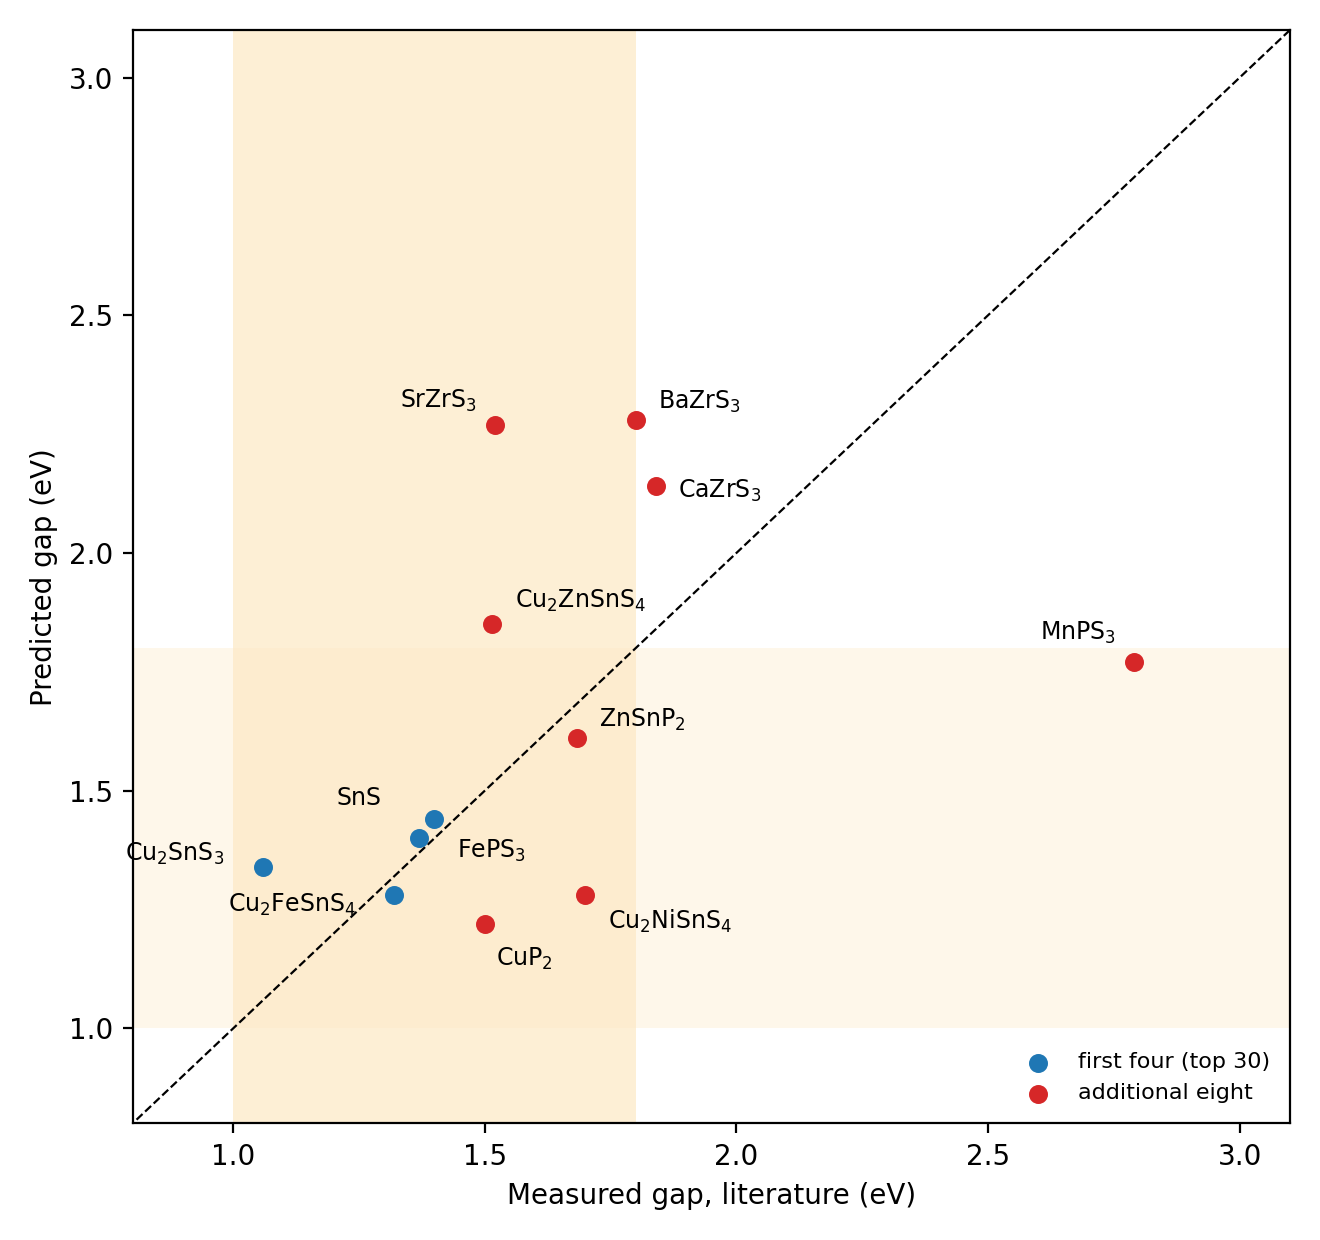
\includegraphics[width=.55\linewidth]{fig_literature_validation.png}\caption{Predicted versus measured literature gaps. Shaded bands mark the 1.0--1.8~eV window.}\label{fig:lit}\end{figure}

\section{Discussion}
Separating metals from non-metals is the main benefit of the two-stage model; it does not make the gap predictions for non-metals clearly better, and its hard rule creates large errors when a non-metal is called a metal, which was most damaging for oxides.
Accuracy varies strongly with chemistry: errors of about 0.335~eV for chalcogenides are small relative to the 0.8~eV width of the target window, whereas errors of 0.694~eV for oxides are not. Because the overall 90th-percentile error of 1.03~eV exceeds that width,
the model cannot confirm that a compound's gap is suitable. It can, however, enrich a list: on held-out chalcogenides and pnictides the top 5\% by window probability contained in-window compounds 3.16 times as often as random selection, which supports its use as a first filter. The stress test shows that these statements hold only for anion families represented in the training data. The literature compilation points the same way: for twelve chalcogenides and pnictides the error (0.34~eV) matched the cross-validated error, every compound with a window probability of at least 0.30 lay in the window, and the misses were zirconium sulfide perovskites that the model placed about 0.5 to 0.75~eV too high. A user should therefore treat a low probability as weak evidence against a candidate, not as exclusion.

Practically, composition-only screening of this kind is a coarse, inexpensive first filter for chalcogenides and pnictides built from abundant elements. It ignores crystal structure, defects, doping, carrier lifetime, stability and processing, all of which determine whether a material works in a device.
Candidates are hypotheses for further calculation or experiment, not demonstrated absorbers.

\paragraph{Limitations.}
(i) Composition alone cannot distinguish polymorphs, defects or measurement conditions, and the compiled data contain label noise. (ii) Chemical-system grouping is a weak test because most systems contain one compound; the family-withholding test is much stricter but also unrealistically severe for most uses.
(iii) The window probability assumes that candidate errors resemble out-of-fold errors. (iv) Negative formation energy is not a proof of stability, and some high-ranked entries (for example Cu$_4$Sn$_{15}$S$_{32}$) may be hypothetical structures; energy above the convex hull would be a better screen. (v) Element abundance values are rounded handbook figures, and the toxicity and cost lists are judgements: Cr, Ni, V and Ba compounds can be hazardous, so ``low-toxicity'' here means only ``not on our exclusion list''.
(vi) The literature comparison covers twelve compounds from a compilation that targeted photovoltaic-relevant materials, with some conflicting reported values (for example MnPS$_3$); it is indicative, not a systematic test. (vii) Models used fixed settings without tuning, so absolute accuracy is not state of the art. (viii) Calibration and enrichment were measured on compounds from the same data set, with 3 fold assignments, so they describe performance on compounds like those in Matbench, not on genuinely new chemistries; the advantage of the window-probability ranking over the two-stage naive ranking is small.

\section{Conclusions}
Under chemical-system cross-validation on 4604 experimental compositions, a two-stage model lowered the overall MAE from 0.474 to 0.384~eV by handling metals separately, without a clear gain for non-metal gaps.
Accuracy was acceptable for chalcogenides and pnictides, poor for oxides and halides, and degraded sharply when an anion family was unseen. A probability-of-window ranking, which was reasonably calibrated and enriched in-window chalcogenides and pnictides 3.16-fold at the top 5\% on held-out data, applied to 8,326 real low-cost compounds yielded 98 candidates above 0.30, and gap predictions for twelve compounds with measured literature values had a mean error of 0.34~eV; none of the candidates has been shown here to be a working absorber. A larger, systematic literature validation and a stability screen based on energy above the convex hull are the most important next steps.

\section*{Data and Code Availability}
The experimental data are the public Matbench \texttt{matbench\_expt\_gap} set; candidate compositions come from the public Materials Project data distributed with \texttt{matminer}. Code, fold assignments, predictions, the literature compilation and all result tables are available at \url{https://github.com/priomdeybd-netizen/earth-abundant-bandgap-screening} and archived on Zenodo (\url{https://doi.org/10.5281/zenodo.23588806}).

\section*{Declaration of AI Assistance}
Generative AI (Anthropic's Claude) was used to help write the analysis code and to draft and edit the manuscript. P.~Dey ran the code and checked the results; A.~Talukder and Y.~Roy checked the cited sources and the reported numbers (see Author Contributions). The authors take full responsibility for the content. AI tools are not listed as authors.

\section*{Author Contributions}
\textbf{Priom Dey:} conceptualization, methodology, software, formal analysis, investigation, data curation, writing -- original draft, visualization, supervision, project administration.
\textbf{Avro Talukder:} validation (checking of cited sources and of reported numbers against the supplied tables), writing -- review and editing.
\textbf{Yuvraj Roy:} validation (checking of cited sources and of reported numbers against the supplied tables), writing -- review and editing.

\section*{Funding}
This research received no specific grant from any funding agency in the public, commercial or not-for-profit sectors.

\section*{Competing Interests}
The authors declare no competing interests.

\appendix
\section{Element abundance values used}
\begin{table}[H]\centering\small\caption{Approximate crustal abundance (mg/kg) of the allowed elements (rounded values following \cite{CRC}).}\label{tab:abund}
\begin{tabular}{lrlrlrlr}\toprule O & 461000 & Si & 282000 & Al & 82300 & Fe & 56300 \\
Ca & 41500 & Na & 23600 & Mg & 23300 & K & 20900 \\
Ti & 5650 & P & 1050 & Mn & 950 & F & 585 \\
Ba & 425 & Sr & 370 & S & 350 & Zr & 165 \\
Cl & 145 & V & 120 & Cr & 102 & Ni & 84 \\
Zn & 70 & Cu & 60 & Li & 20 & N & 19 \\
Br & 2.4 & Sn & 2.3 &  &  &  &  \\
\bottomrule\end{tabular}\end{table}

\begin{thebibliography}{99}\small
\bibitem{Dunn2020} A.~Dunn, Q.~Wang, A.~Ganose, D.~Dopp, A.~Jain, Benchmarking materials property prediction methods: the Matbench test set and Automatminer reference algorithm, \emph{npj Comput.\ Mater.} \textbf{6}, 138 (2020).
\bibitem{Ward2016} L.~Ward, A.~Agrawal, A.~Choudhary, C.~Wolverton, A general-purpose machine learning framework for predicting properties of inorganic materials, \emph{npj Comput.\ Mater.} \textbf{2}, 16028 (2016).
\bibitem{Zhuo2018} Y.~Zhuo, A.~Mansouri Tehrani, J.~Brgoch, Predicting the band gaps of inorganic solids by machine learning, \emph{J.\ Phys.\ Chem.\ Lett.} \textbf{9}, 1668 (2018).
\bibitem{Meredig2018} B.~Meredig et al., Can machine learning identify the next high-temperature superconductor? Examining extrapolation performance for materials discovery, \emph{Mol.\ Syst.\ Des.\ Eng.} \textbf{3}, 819 (2018).
\bibitem{Ong2013} S.~P.~Ong et al., Python Materials Genomics (pymatgen), \emph{Comput.\ Mater.\ Sci.} \textbf{68}, 314 (2013).
\bibitem{Ward2018matminer} L.~Ward et al., Matminer: an open source toolkit for materials data mining, \emph{Comput.\ Mater.\ Sci.} \textbf{152}, 60 (2018).
\bibitem{Pedregosa2011} F.~Pedregosa et al., Scikit-learn: machine learning in Python, \emph{J.\ Mach.\ Learn.\ Res.} \textbf{12}, 2825 (2011).
\bibitem{Breiman2001} L.~Breiman, Random forests, \emph{Mach.\ Learn.} \textbf{45}, 5 (2001).
\bibitem{Jain2013} A.~Jain et al., Commentary: The Materials Project: a materials genome approach to accelerating materials innovation, \emph{APL Mater.} \textbf{1}, 011002 (2013).
\bibitem{SQ1961} W.~Shockley, H.~J.~Queisser, Detailed balance limit of efficiency of p--n junction solar cells, \emph{J.\ Appl.\ Phys.} \textbf{32}, 510 (1961).
\bibitem{CRC} W.~M.~Haynes (ed.), \emph{CRC Handbook of Chemistry and Physics}, CRC Press (current edition; abundance of the elements in the Earth's crust).
\bibitem{Reddy2006} N.~Koteeswara Reddy, K.~Ramesh, R.~Ganesan, K.~T.~Ramakrishna Reddy, K.~R.~Gunasekhar, E.~S.~R.~Gopal, Synthesis and characterisation of co-evaporated tin sulphide thin films, \emph{Appl.\ Phys.\ A} \textbf{83}, 133 (2006). doi:10.1007/s00339-005-3475-y
\bibitem{Marquez2016} J.~Marquez Prieto, S.~Levcenko, J.~Just, H.~Hampel, I.~Forbes, N.~Pearsall, T.~Unold, Earth abundant thin film solar cells from co-evaporated Cu$_2$SnS$_3$ absorber layers, \emph{J.\ Alloys Compd.} \textbf{689}, 182 (2016). doi:10.1016/j.jallcom.2016.07.293
\bibitem{Hou2017} H.~Hou, H.~Guan, L.~Li, Synthesis of Cu$_2$FeSnS$_4$ thin films with stannite and wurtzite structure directly on glass substrates via the solvothermal method, \emph{J.\ Mater.\ Sci.: Mater.\ Electron.} \textbf{28}, 7745 (2017). doi:10.1007/s10854-017-6469-6
\bibitem{Budniak2022} A.~K.~Budniak, S.~J.~Zelewski, M.~Birowska, T.~Wo\'zniak, T.~Bendikov, Y.~Kauffmann, Y.~Amouyal, R.~Kudrawiec, E.~Lifshitz, Spectroscopy and structural investigation of iron phosphorus trisulfide -- FePS$_3$, \emph{Adv.\ Opt.\ Mater.} \textbf{10}, 2102489 (2022); arXiv:2108.01742.
\bibitem{Zhang2009} X.~Zhang, X.~Shi, W.~Ye et al., Electrochemical deposition of quaternary Cu$_2$ZnSnS$_4$ thin films as potential solar cell material, \emph{Appl.\ Phys.\ A} \textbf{94}, 381 (2009). doi:10.1007/s00339-008-4815-5
\bibitem{Jiang2012} F.~Jiang, H.~Shen, W.~Wang,  Optical and electrical properties of Cu$_2$ZnSnS$_4$ film prepared by sulfurization method, \emph{J.\ Electron.\ Mater.} \textbf{41}, 2204 (2012). doi:10.1007/s11664-012-2112-8
\bibitem{Beraich2020} M.~Beraich, M.~Taibi, A.~Guenbour et al., Synthesis of tetragonal Cu$_2$NiSnS$_4$ thin film via low-cost electrodeposition method: effect of Ni$^{2+}$ molarity, \emph{J.\ Electron.\ Mater.} \textbf{49}, 728 (2020). doi:10.1007/s11664-019-07707-4
\bibitem{StJean2010} P.~St-Jean, G.~A.~Seryogin, S.~Francoeur, Band gap of sphalerite and chalcopyrite phases of epitaxial ZnSnP$_2$, \emph{Appl.\ Phys.\ Lett.} \textbf{96}, 231913 (2010). doi:10.1063/1.3442917
\bibitem{Crovetto2022} A.~Crovetto, D.~Kojda, F.~Yi, K.~N.~Heinselman, D.~A.~LaVan, K.~Habicht, T.~Unold, A.~Zakutayev, Crystallize it before it diffuses: kinetic stabilization of thin-film phosphorus-rich semiconductor CuP$_2$, \emph{J.\ Am.\ Chem.\ Soc.} \textbf{144}, 13334 (2022). doi:10.1021/jacs.2c04868
\bibitem{Gupta2019} T.~Gupta, D.~Ghoshal, A.~Yoshimura et al., An environmentally stable and lead-free chalcogenide perovskite, \emph{Adv.\ Funct.\ Mater.} \textbf{30}, 2001387 (2020); arXiv:1912.07082.
\bibitem{Wei2019} X.~Wei, H.~Hui, C.~Zhao et al., Realization of BaZrS$_3$ chalcogenide perovskite thin films for optoelectronics, \emph{Nano Energy} \textbf{68}, 104317 (2020); arXiv:1910.04978.
\bibitem{Niu2017} S.~Niu, H.~Huyan, Y.~Liu et al., Bandgap control via structural and chemical tuning of transition metal perovskite chalcogenides, \emph{Adv.\ Mater.} \textbf{29}, 1604733 (2017). doi:10.1002/adma.201604733
\bibitem{Zhao2025} P.~Zhao, L.~Yang, S.~Kong et al., Impact of sulfurization temperature on the formation and properties of chalcogenide perovskites, \emph{Molecules} \textbf{30}, 1198 (2025). doi:10.3390/molecules30061198
\bibitem{Harchol2024} A.~Harchol et al., Tuning magnetic and optical properties in Mn$_x$Zn$_{1-x}$PS$_3$ single crystals by the alloying composition, arXiv:2404.07643 (2024).
\end{thebibliography}
\end{document}
